\section{Paper 6}
\subsection{\emph{"Coarse-to-Fine Semantic Segmentation From Image-Level Labels"}}

\begin{frame}{INTRODUCTION}
    Weakly supervised and semi-supervised methods are used to achieve 
    semantic segmentation. These methods need techniques that are capable 
    of producing useful labels in order to train the models. Two types of 
    techniques that produce labels are: \emph{Image-level labels} (categories) and 
    \emph{Object-level labels} (bounding boxes). In the following paper, the use of 
    the first technique prevails over the second because it is more accurate. 
    The proposed framework has the task of training a model that only 
    depends on image category level annotations. The final goal is to be able 
    to recognize different objects, in the foreground, belonging to different 
    categories.
\end{frame}

\begin{frame}{RELATED WORK}
    The following framework can be used for both semantic segmentation 
    and foreground object segmentation. There are various models proposed 
    at the state of the art that carry out a different semantic segmentation 
    and a different foreground segmentation.
    \begin{table}[h!]
        \begin{adjustbox}{max width=\textwidth}
        \begin{tabular}{|p{6cm}|p{6cm}|}
            \hline
            \centering
            \bfseries{Semantic Segmentation Methods} &  ~\bfseries{Foreground Segmentation Methods} \\
            \hline
            \begin{enumerate}
                \item \emph{Fully Supervised Pixel-Wise Annotation-Based Methods}: trained with 
                pixel-wise labels annotated by people.
                \item \emph{Weakly Supervised Object-level Annotation-Based-Methods}: trained with 
                methods such as object-level annotations based on the use of bounding 
                boxes.
                \item \emph{Weakly Supervised Image-Level Annotation-Based Methods}: trained 
                with image category labels.
            \end{enumerate}
            & 
            \begin{enumerate}
                \item \emph{Joint segmentation-based Methods}: used prior knowledge as supervision.
                \item \emph{Saliency prediction-based Methods}: identify regions present in the human 
                visual scene.
                \item \emph{Object proposal-based Methods}: locate all objects in images.
            \end{enumerate}\\
            \hline
        \end{tabular}
        \end{adjustbox}
    \end{table}
\end{frame}

\begin{frame}{THE PROPOSED APPROACH - 3 Steps}
    The work performed by the model is divided into three steps: \emph{coarse mask generation}, \emph{coarse mask enhancement}, and \emph{recursive mask refinement}.
    \begin{figure}[h!]
        \centering
        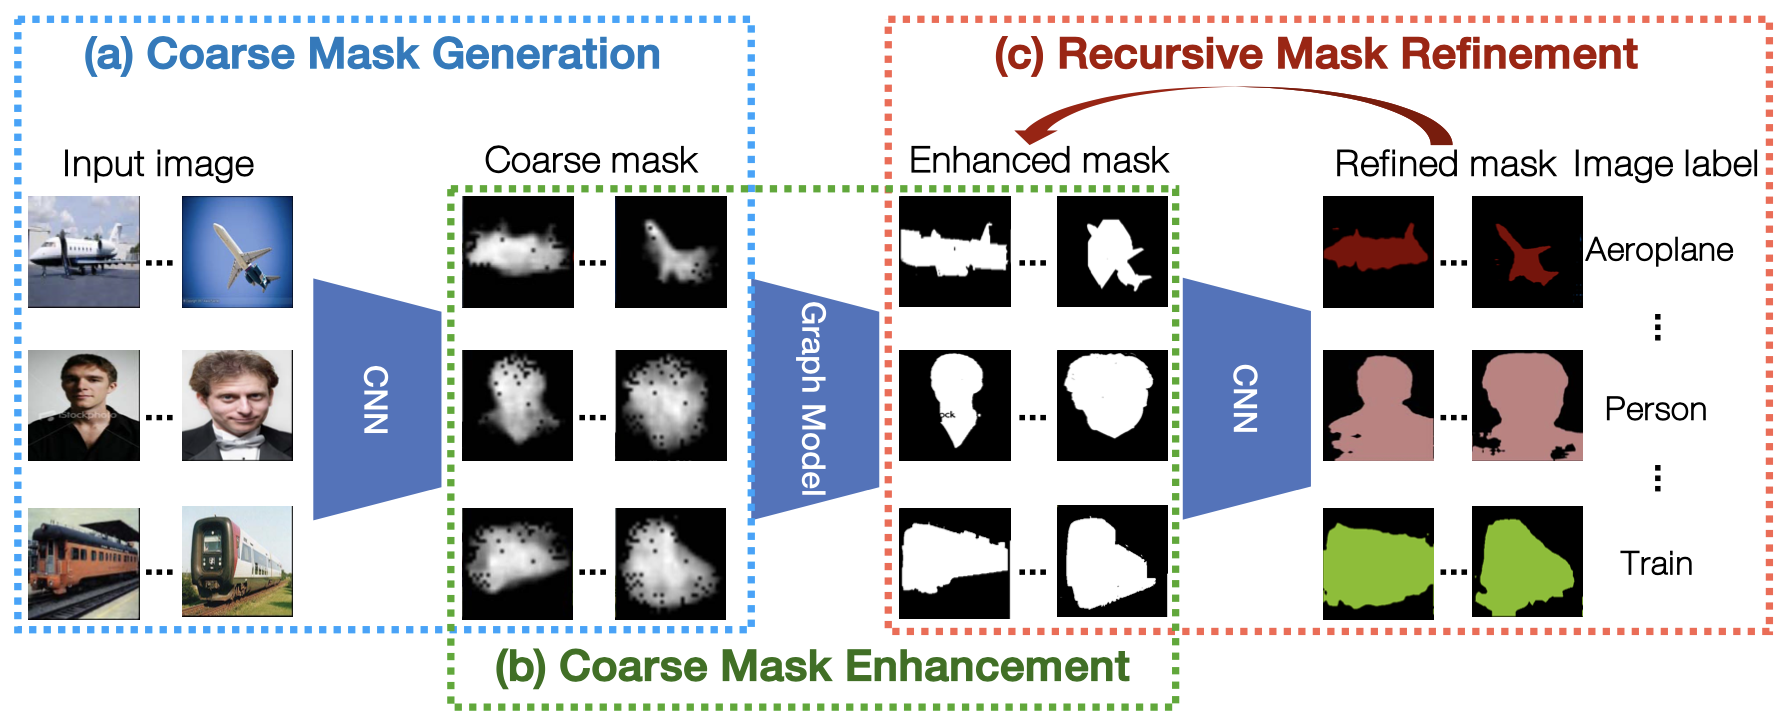
\includegraphics[width = 1 \linewidth]{images/paper6/step.png}
        \centering
        \caption{Steps of the proposed method.}
    \end{figure}
\end{frame}

\begin{frame}{THE PROPOSED APPROACH - \emph{Coarse Mask Generation}}
    \begin{minipage}{\linewidth}
        \centering
        \begin{minipage}{0.45\linewidth}
            A CNN network\footnotemark ~is used to be able 
            to extract a first coarse mask. 
            Unfortunately, as can be seen in 
            the image, the generated masks 
            appear to be inaccurate and do 
            not comply with the position of 
            the underlying object.
        \end{minipage}
        \hspace{0.05\linewidth}
        \begin{minipage}{0.45\linewidth}
            \begin{figure}[h!]
                \centering
                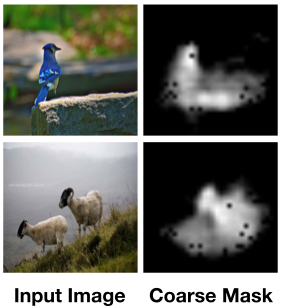
\includegraphics[width = 1 \linewidth]{images/paper6/coarse mask.png}
                \centering
            \end{figure}
        \end{minipage}
    \end{minipage}
    \footnotetext{I. Croitoru, S.-V. Bogolin, and M. Leordeanu, “Unsupervised learning from video to detect foreground objects in single images,” in Proc. IEEE Int. Conf. Comput. Vis. (ICCV), Oct. 2017, pp. 4335–4343.}
\end{frame}

\begin{frame}{THE PROPOSED APPROACH - \emph{Coarse Mask Enhancement}}
    To carry out the enhanced coarse mask, the unsupervised GrubCut 
    model\footnotemark ~is used. To achieve mask optimization, the 
    method performs the following two steps:
    \begin{minipage}{\linewidth}
        \centering
        \begin{minipage}{0.45\linewidth}
            \begin{enumerate}
                \item search for the smallest bounding box inside the mask.
                \item enhance the mask based on the previously created bounding box and on the RGB image.
            \end{enumerate}
        \end{minipage}
        \hspace{0.05\linewidth}
        \begin{minipage}{0.45\linewidth}
            \begin{figure}[h!]
                \centering
                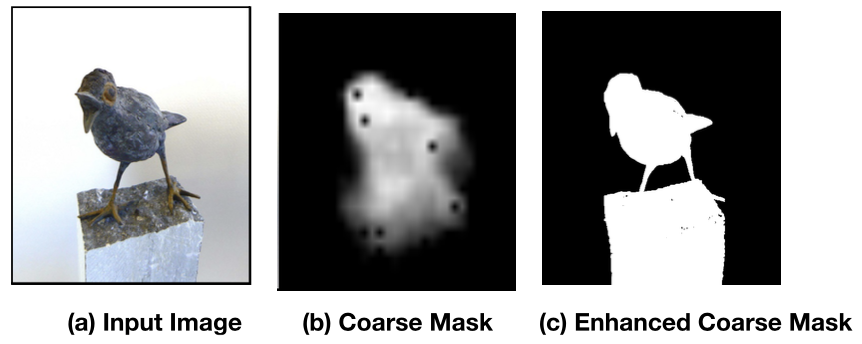
\includegraphics[width = 1.2 \linewidth]{images/paper6/enhancement.png}
                \centering
            \end{figure}
        \end{minipage}
    \end{minipage}
    \footnotetext{C. Rother, V. Kolmogorov, and A. Blake, “GrabCut: Interactive foreground extraction using iterated graph cuts,” ACM Trans. Graph., vol. 23, no. 3, pp. 309–314, 2004.}
\end{frame}

\begin{frame}{THE PROPOSED APPROACH - \emph{Recursive Mask Refinement}}
    A network called DeepLab \footfullcite{0876055502} is used for semantic segmentation. This 
    network uses the mask generated by the GrubCut method and, through a 
    comparison on the original image, produces a new better mask that will 
    be used as a new training set. The best mask will be obtained after a 
    maximum of 5 training rounds.
    \begin{figure}[h!]
        \centering
        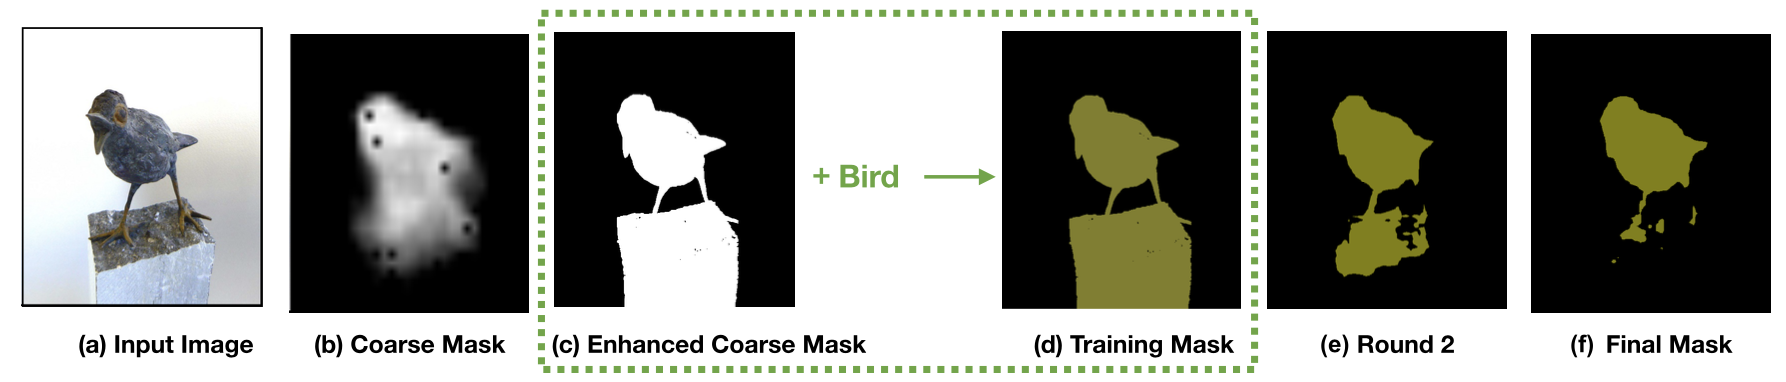
\includegraphics[width = 1 \linewidth]{images/paper6/DeepLab.png}
        \centering
    \end{figure}
\end{frame}

\begin{frame}{THE PROPOSED APPROACH - \emph{Extended the Proposed Framework to Foreground Segmentation}}
    
\end{frame}




